% $Header: /cvsroot/latex-beamer/latex-beamer/solutions/generic-talks/generic-ornate-15min-45min.en.tex,v 1.5 2007/01/28 20:48:23 tantau Exp $

\documentclass[12pt]{beamer}
%\documentclass[12pt,handout]{beamer}

% This file is a solution template for:

% - Giving a talk on some subject.
% - The talk is between 15min and 45min long.
% - Style is ornate.



% Copyright 2004 by Till Tantau <tantau@users.sourceforge.net>.
%
% In principle, this file can be redistributed and/or modified under
% the terms of the GNU Public License, version 2.
%
% However, this file is supposed to be a template to be modified
% for your own needs. For this reason, if you use this file as a
% template and not specifically distribute it as part of a another
% package/program, I grant the extra permission to freely copy and
% modify this file as you see fit and even to delete this copyright
% notice.


\mode<presentation>
{
  \usetheme{default}
  % or ...

  \setbeamercovered{transparent}
  % or whatever (possibly just delete it)
}
\setbeamertemplate{navigation symbols}{}%remove navigation symbols


\usepackage[english]{babel}
% or whatever

\usepackage[latin1]{inputenc}
% or whatever

\usepackage{times}
\usepackage{sansmathfonts}
\usepackage[T1]{fontenc}
% Or whatever. Note that the encoding and the font should match. If T1
% does not look nice, try deleting the line with the fontenc.


\title%[Short Paper Title] % (optional, use only with long paper titles)
{}

\subtitle
{} % (optional)

\author%[Author, Another] (optional, use only with lots of authors)
{Ben Holder}%{F.~Author\inst{1} \and S.~Another\inst{2}}
% - Use the \inst{?} command only if the authors have different
%   affiliation.

%\institute[Universities of Somewhere and Elsewhere] % (optional, but mostly needed)
%{
%  \inst{1}%
%  Department of Computer Science\\
%  University of Somewhere
%  \and
%  \inst{2}%
%  Department of Theoretical Philosophy\\
%  University of Elsewhere}
%% - Use the \inst command only if there are several affiliations.
%% - Keep it simple, no one is interested in your street address.

\date%[Short Occasion] % (optional)
{}

\subject{Talks}
% This is only inserted into the PDF information catalog. Can be left
% out.



% If you have a file called "university-logo-filename.xxx", where xxx
% is a graphic format that can be processed by latex or pdflatex,
% resp., then you can add a logo as follows:

% \pgfdeclareimage[height=0.5cm]{university-logo}{university-logo-filename}
% \logo{\pgfuseimage{university-logo}}



% Delete this, if you do not want the table of contents to pop up at
% the beginning of each subsection:
%\AtBeginSubsection[]
%{
%  \begin{frame}<beamer>{Outline}
%    \tableofcontents[currentsection,currentsubsection]
%  \end{frame}
%}


% If you wish to uncover everything in a step-wise fashion, uncomment
% the following command:

%\beamerdefaultoverlayspecification{<+->}

\usepackage{enumerate}
\usepackage{amsmath}
\usepackage{amssymb}
\usepackage[amssymb]{SIunits}
\usepackage{url}
\usepackage{hyperref}
\usepackage[normalem]{ulem}


\setbeamercovered{invisible}

\hypersetup{
    colorlinks=true,     % false: boxed links; true: colored links
    linkcolor=red,       % color of internal links
    citecolor=blue,      % color of links to bibliography
    filecolor=blue,      % color of file links
    urlcolor=blue        % color of external links
}


\begin{document}

%\begin{frame}
%  \titlepage
%\end{frame}

%%%%%%%%%%%%%%%%%%%%%%%%%%%%%%%%%%%%%%
\begin{frame}{Announcements}
	%
	\begin{itemize}
	\addtolength{\itemsep}{0.5\baselineskip}
	\item Any questions/issues?
	\item \underline{Schedule}:
		%
		\begin{itemize}
		\item[]{\bf Today (Follow-up)}: Milankovitch cycles and observation in paleodata
		\item[]{\bf Today (New)}: ``Climate sensitivity'' --- how precisely does additional $\text{CO}_2$  cause warming
		\item[]{\bf Tomorrow (Lab)}: Absorption by $\text{CO}_2$.
		\item[]{\bf Thursday (Discussion)}: Absorption line of $\text{CO}_2$ and temperature increase.
		\item[] {\bf Next Week}: Timescales of climate change.
		\end{itemize}
		%
	\end{itemize}

\end{frame}
%%%%%%%%%%%%%%%%%%%%%%%%%%%%%%%%%%%%%%
\begin{frame}{Today's Reading Quiz (3 min)}


	
\vspace{1cm}

On your own sheet of paper\ldots

\vspace{0.5cm}

{\bf Briefly explain \underline{saturation} in terms of the ``murky pond.''  Then say a few words about saturation in the absorption lines of $\text{CO}_2$ and/or methane.}
\vspace{0.5cm}

Turn in to Blackboard as scanned pdf (or image is fine).

\end{frame}
%%%%%%%%%%%%%%%%%%%%%%%%%%%%%%%%%%%%%%
\begin{frame}{Orbital effects on solar radiation}


\begin{center}
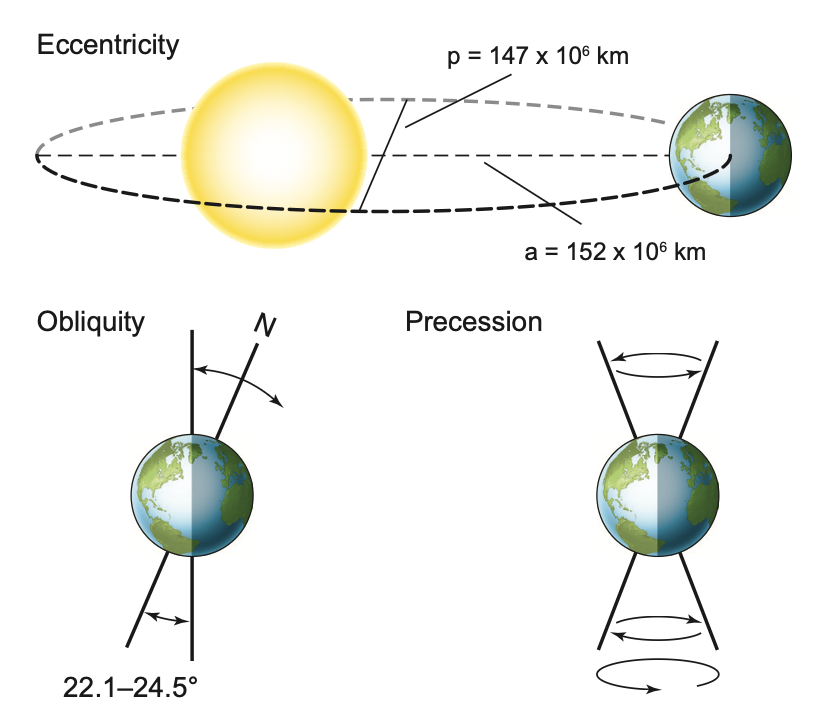
\includegraphics[width=0.8\textwidth]{images/mathez_fig7-5.png}
\end{center}

\href{https://science.nasa.gov/science-research/earth-science/milankovitch-orbital-cycles-and-their-role-in-earths-climate/}{NASA videos showing each type of change}

\end{frame}
%%%%%%%%%%%%%%%%%%%%%%%%%%%%%%%%%%%%%%
\begin{frame}{Orbital effects on solar radiation}


\begin{center}
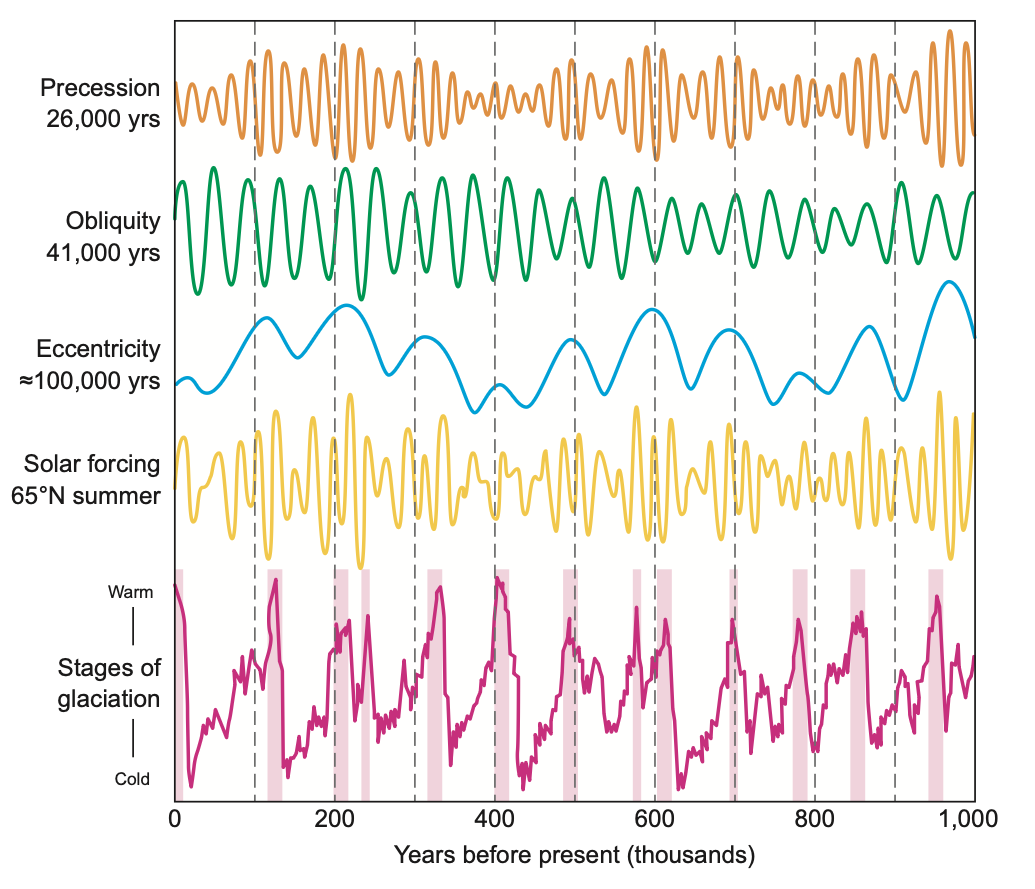
\includegraphics[width=0.8\textwidth]{images/mathez_fig7-9.png}
\end{center}

\end{frame}
%%%%%%%%%%%%%%%%%%%%%%%%%%%%%%%%%%%%%%
\begin{frame}{}

\begin{center}
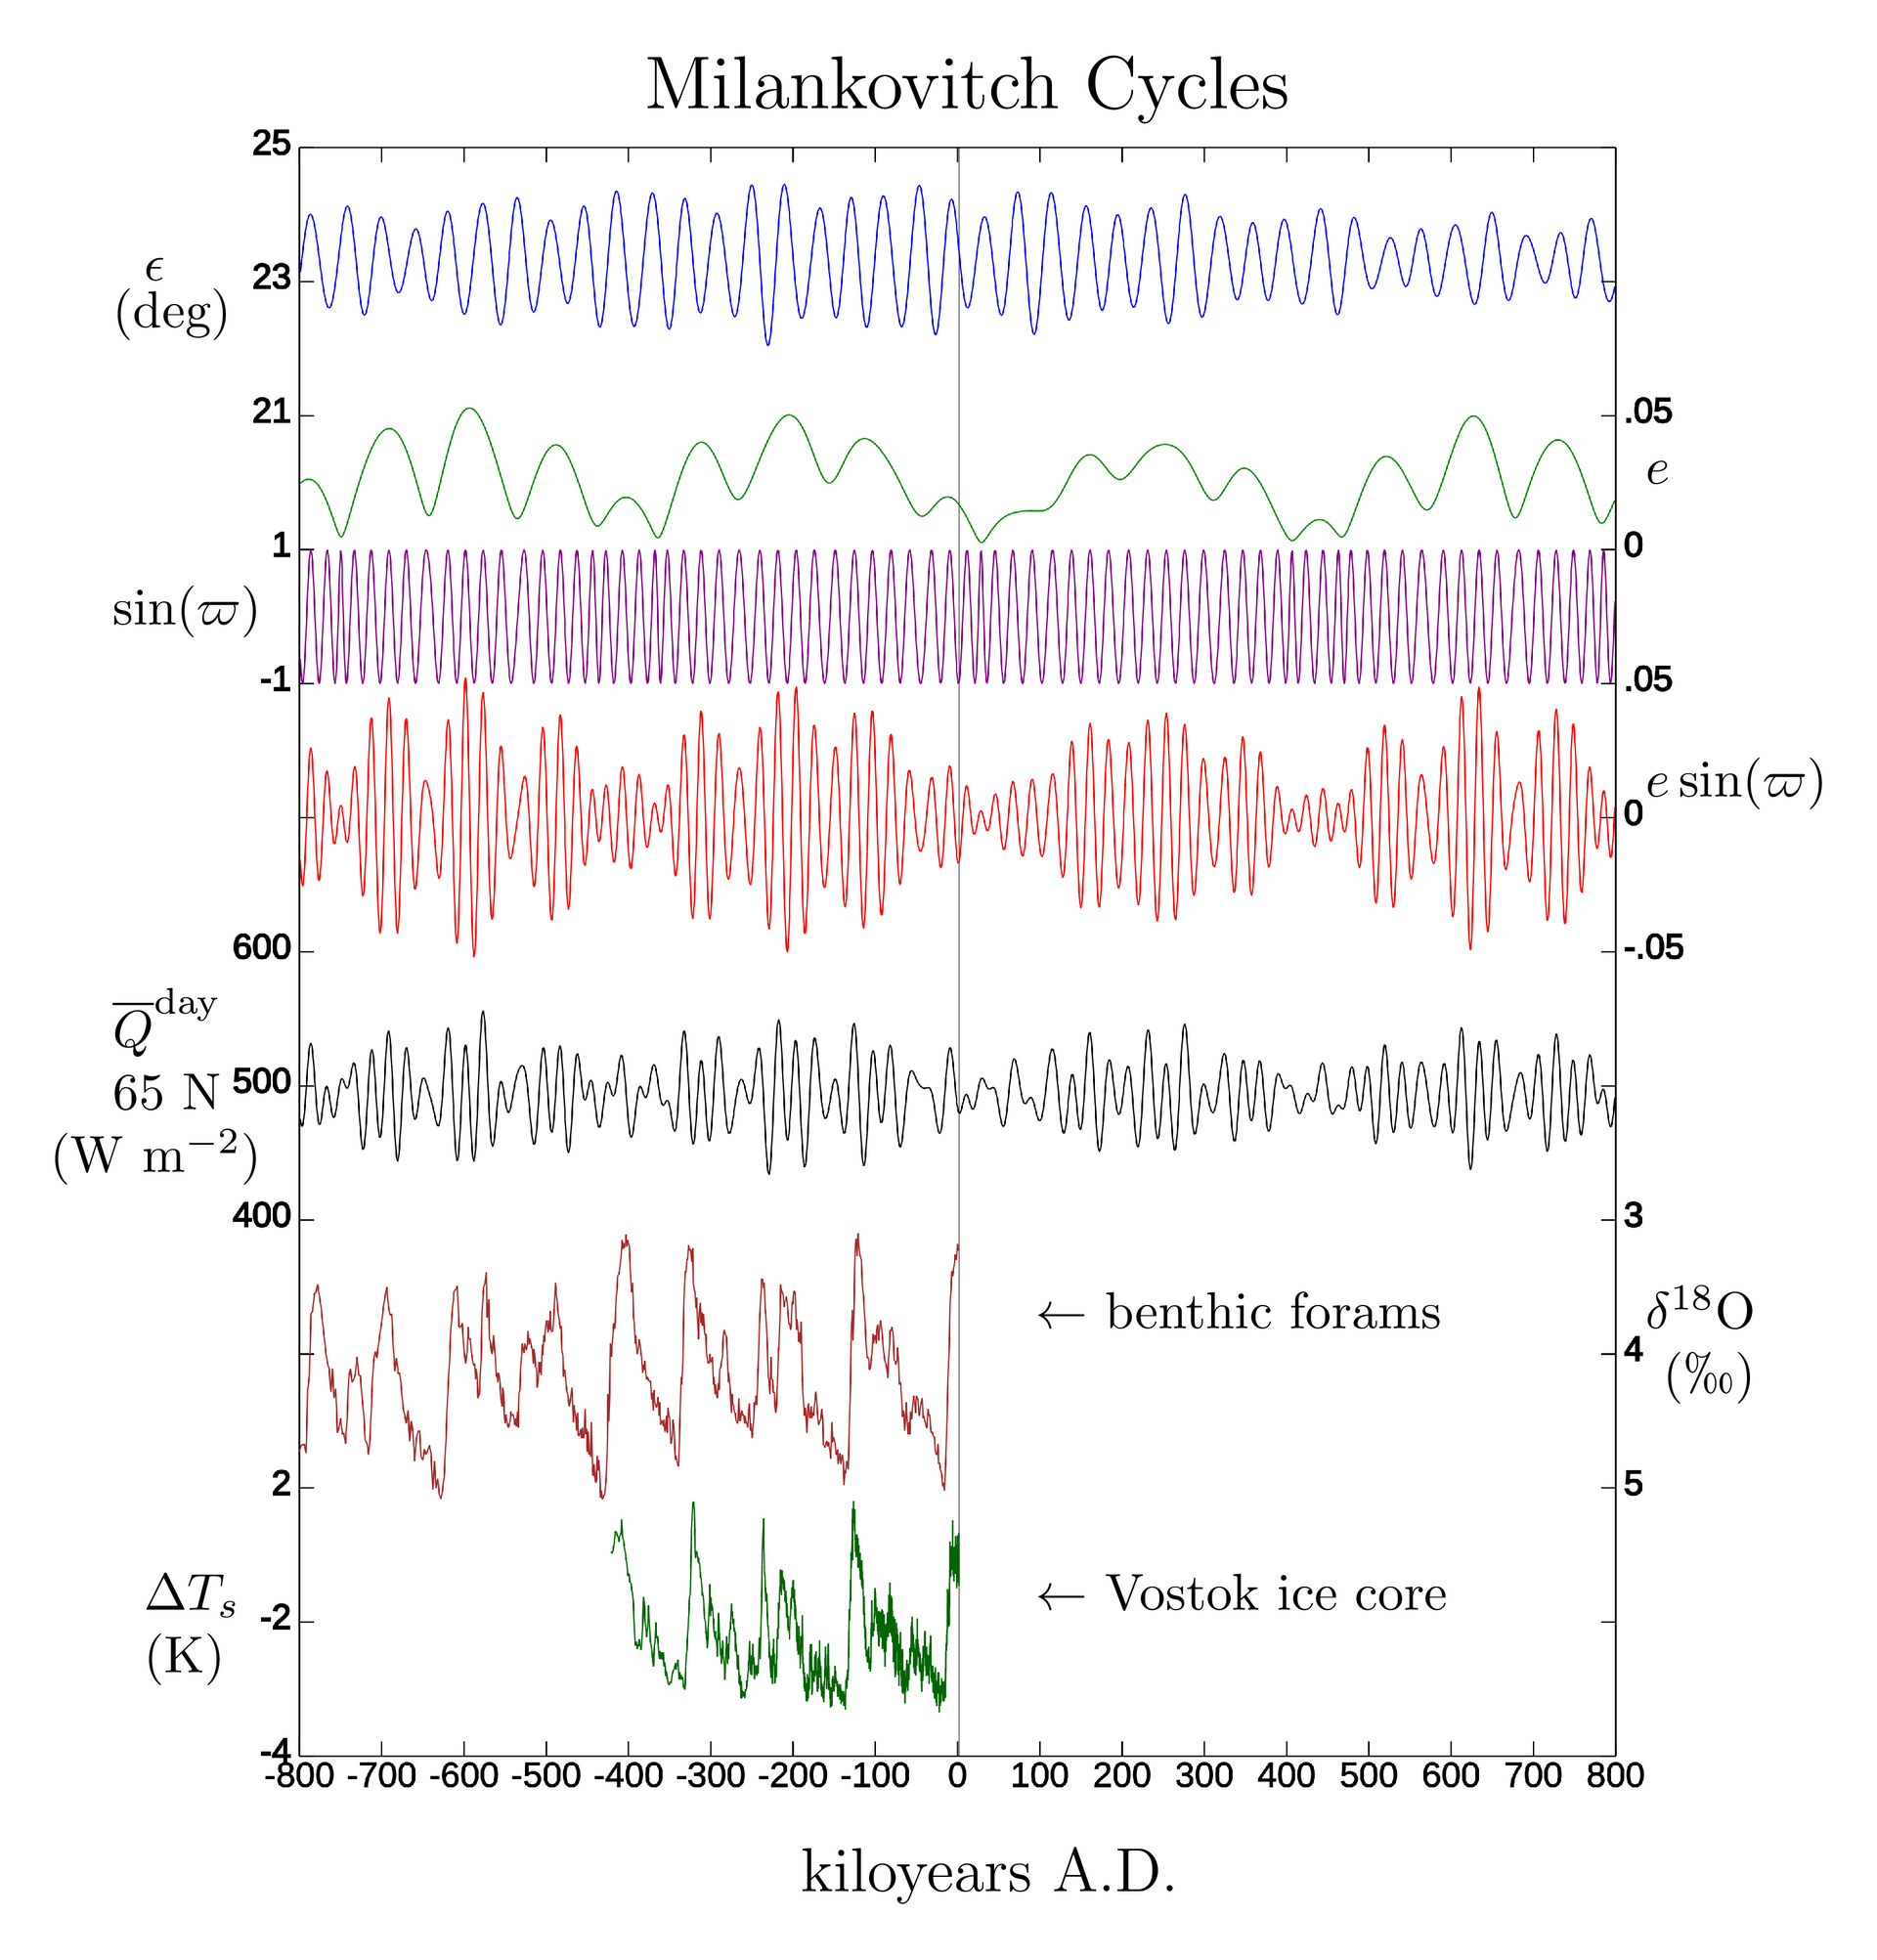
\includegraphics[width=0.75\textwidth]{images/milankovitch_wikimedia-incredio.png}
\end{center}

\end{frame}
%%%%%%%%%%%%%%%%%%%%%%%%%%%%%%%%%%%%%%
\begin{frame}{Paleotemperature Data}

{\small The ``Vostok'' ice cores from Antartica reveals temperature proxy data and direct measurements of gas concentrations over 400,000 years from trapped bubbles.}


\begin{center}
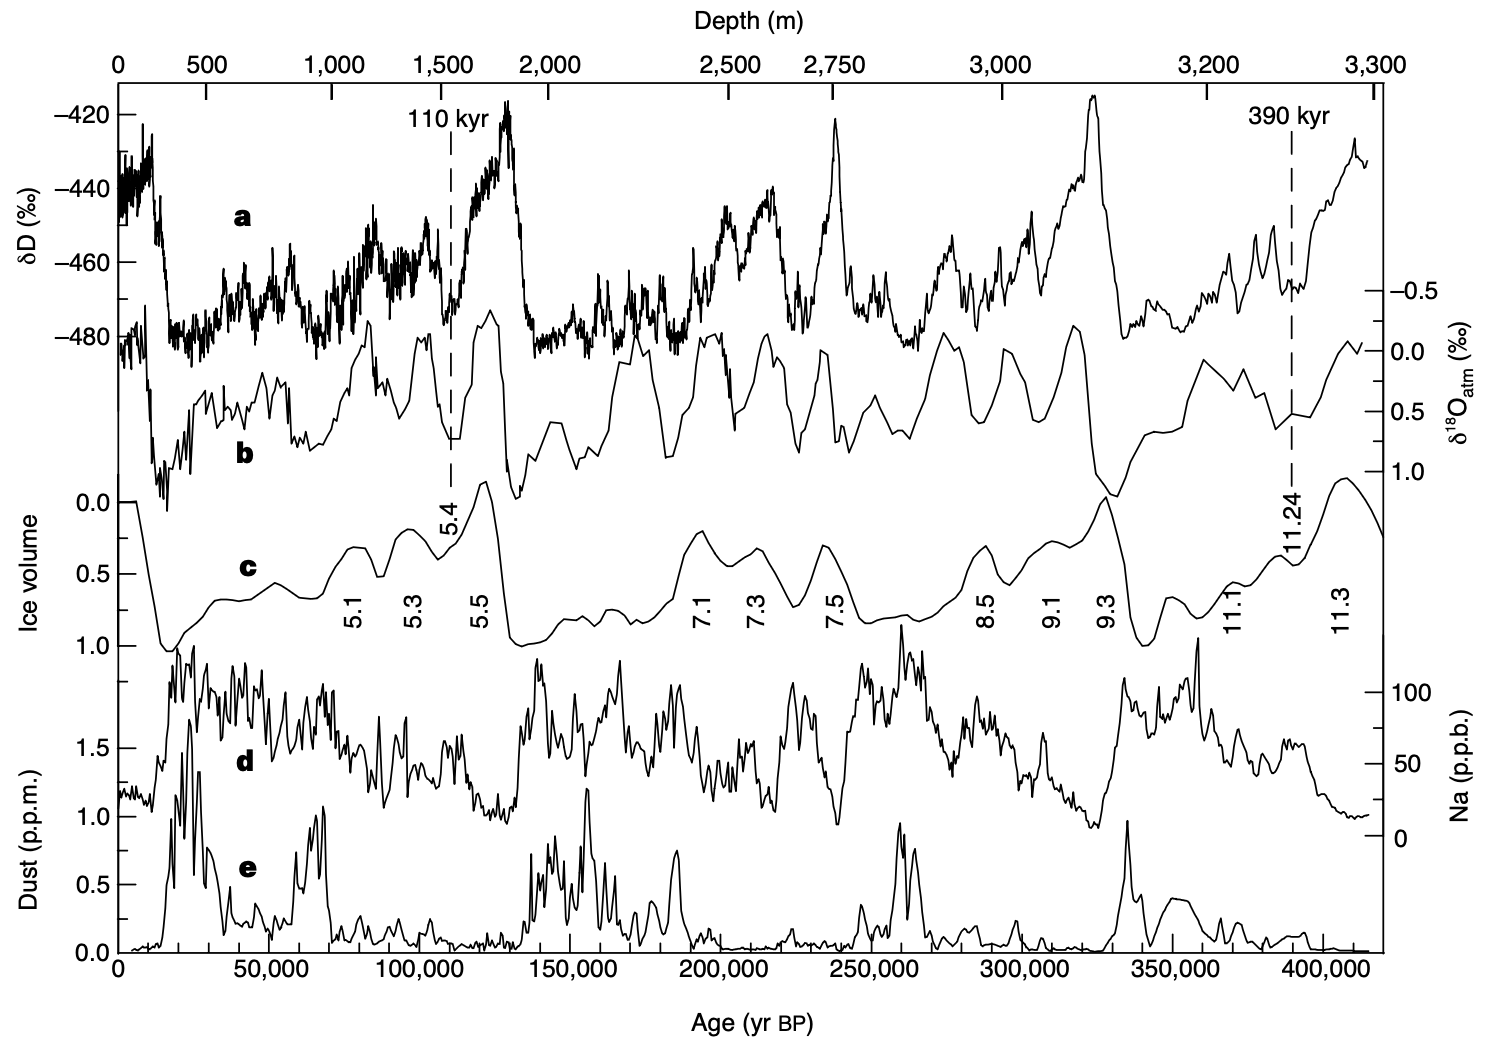
\includegraphics[width=0.68\textwidth]{images/petit-etal_fig2_no-caption.png}
\end{center}


\begin{equation*}
\Delta T = \frac{\delta \text{D} - 8\, \delta^{18} \text{O}}{9} \quad \text{\small (how temperature is estimated)}
\end{equation*}
\end{frame}
%%%%%%%%%%%%%%%%%%%%%%%%%%%%%%%%%%%%%%
\begin{frame}{Paleotemperature Data}

Overplotting the Milankovitch cycle prediction of solar flux makes some tantalizing (but not completely clear) connections.

\begin{center}
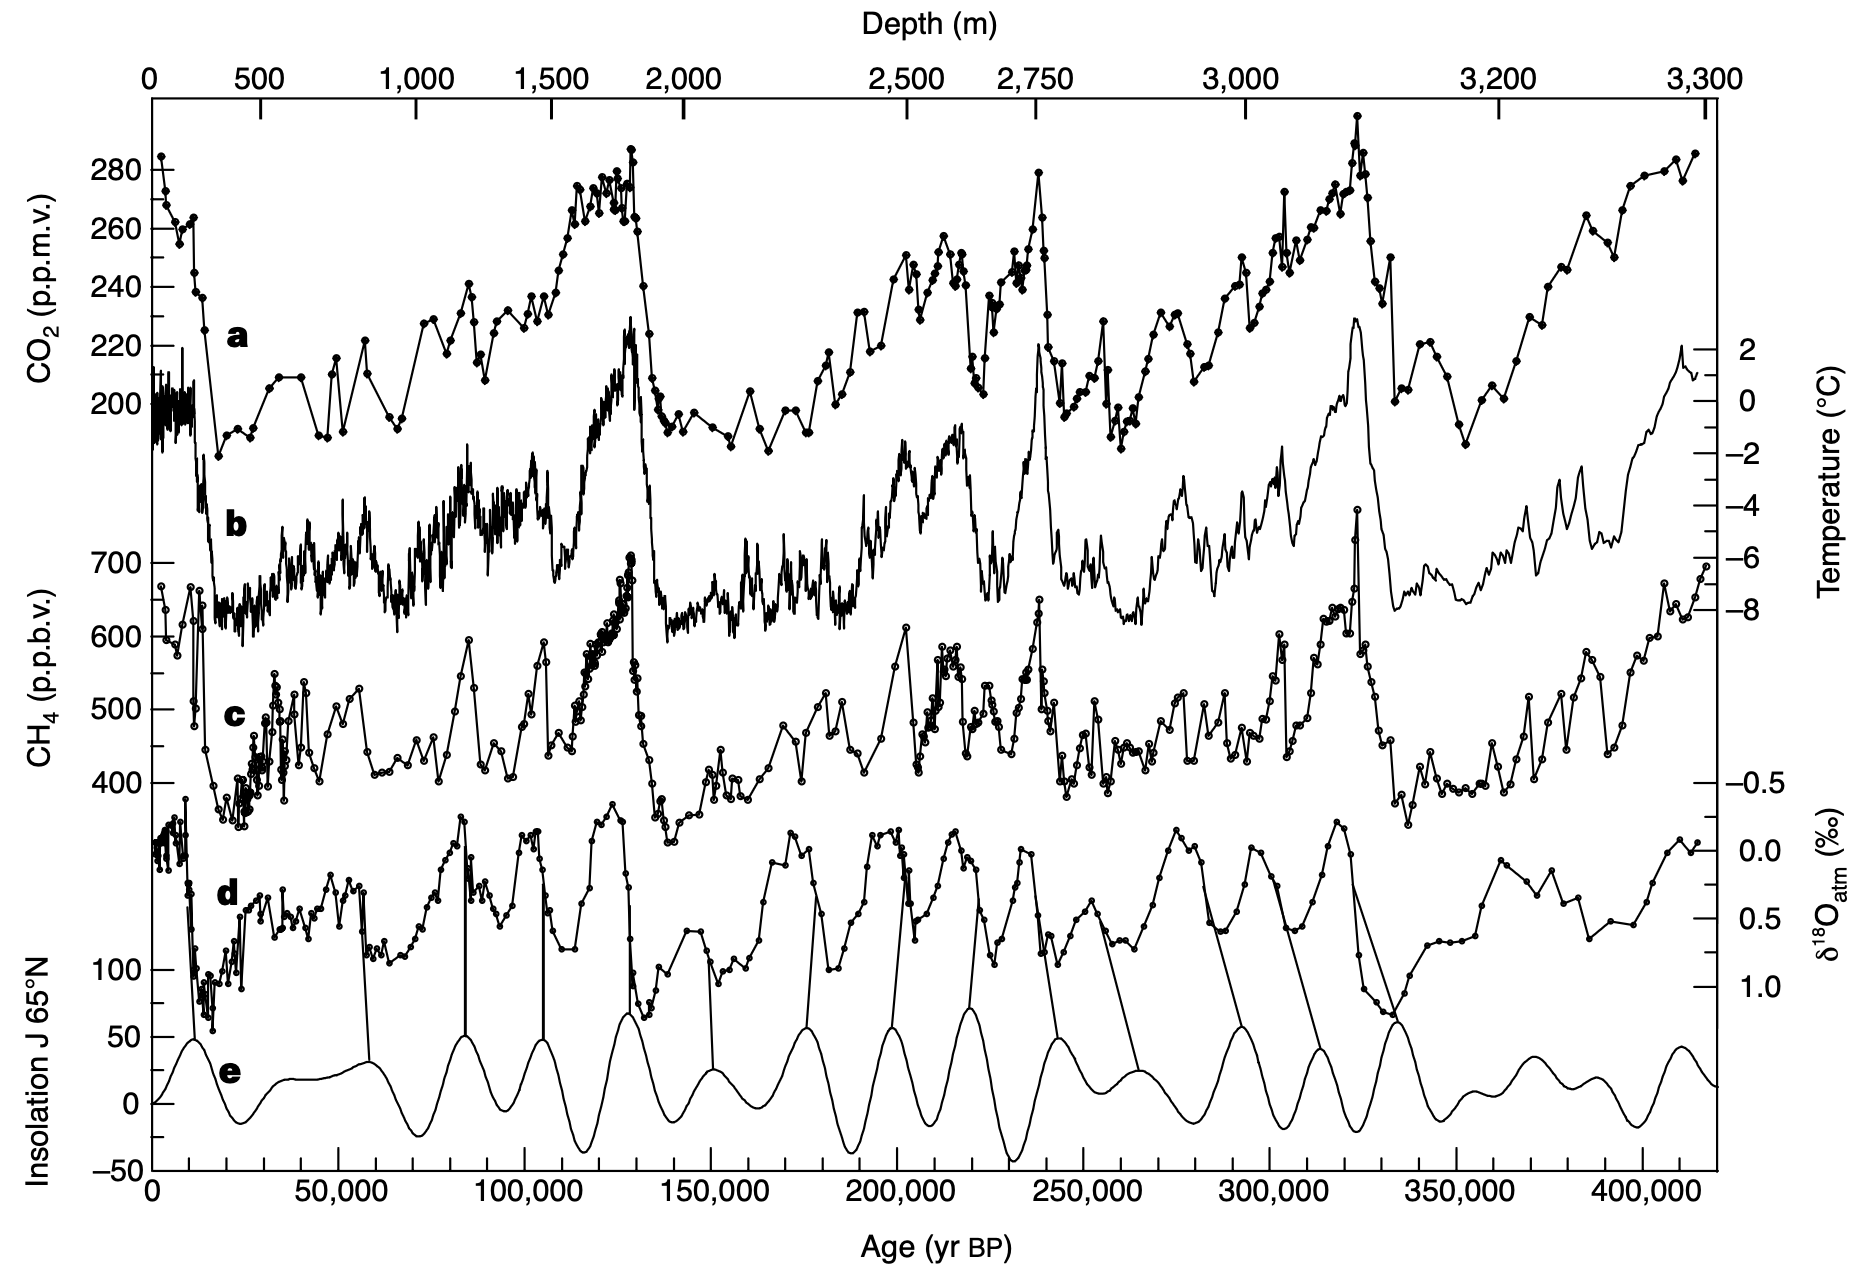
\includegraphics[width=0.9\textwidth]{images/petit-etal_fig3_no-caption.png}
\end{center}

\end{frame}
%%%%%%%%%%%%%%%%%%%%%%%%%%%%%%%%%%%%%%
\begin{frame}{Climate Sensitivity}

The term {\bf climate sensitivity} is often used by climate scientists in two ways:
	%
	\begin{itemize}
	\item The effect on temperature by a doubling of $\text{CO}_2$ in the atmosphere.
	\item The general connection between changes in $\text{CO}_2$ concentration (and other greenhouse gases) and the accompanying temperature rise.
	\end{itemize}
	%
This week we would like to explore exactly how additional $\text{CO}_2$ in the atmosphere, which causes additional {\em absorption} of the Earth surface's infrared blackbody to space, changes the equilibrium temperature of the Earth's surface.

\end{frame}
%%%%%%%%%%%%%%%%%%%%%%%%%%%%%%%%%%%%%%
\begin{frame}{``Greenhouse Gases'' reading (Archer, Chapter 4)}

\begin{itemize}
\item A marked-up version of the chapter identifies key points of review --- from our prior studies of blackbody radiation, absorption of infrared light due to changes in dipole moments, absorption lines in BB spectra, and the connction between temperature and altitude (the {\em lapse rate}) --- and highlights of new information.
\item Today in class we'll go quickly through the review points and then try to understand the key points that the figures convey.
\item In Discussion on Thursday you will do some of this analysis yourself on your own blackbody spectrum curves.
\end{itemize}

\end{frame}
%%%%%%%%%%%%%%%%%%%%%%%%%%%%%%%%%%%%%%
\begin{frame}{Blackbody curves, absorption line saturation}



\begin{center}
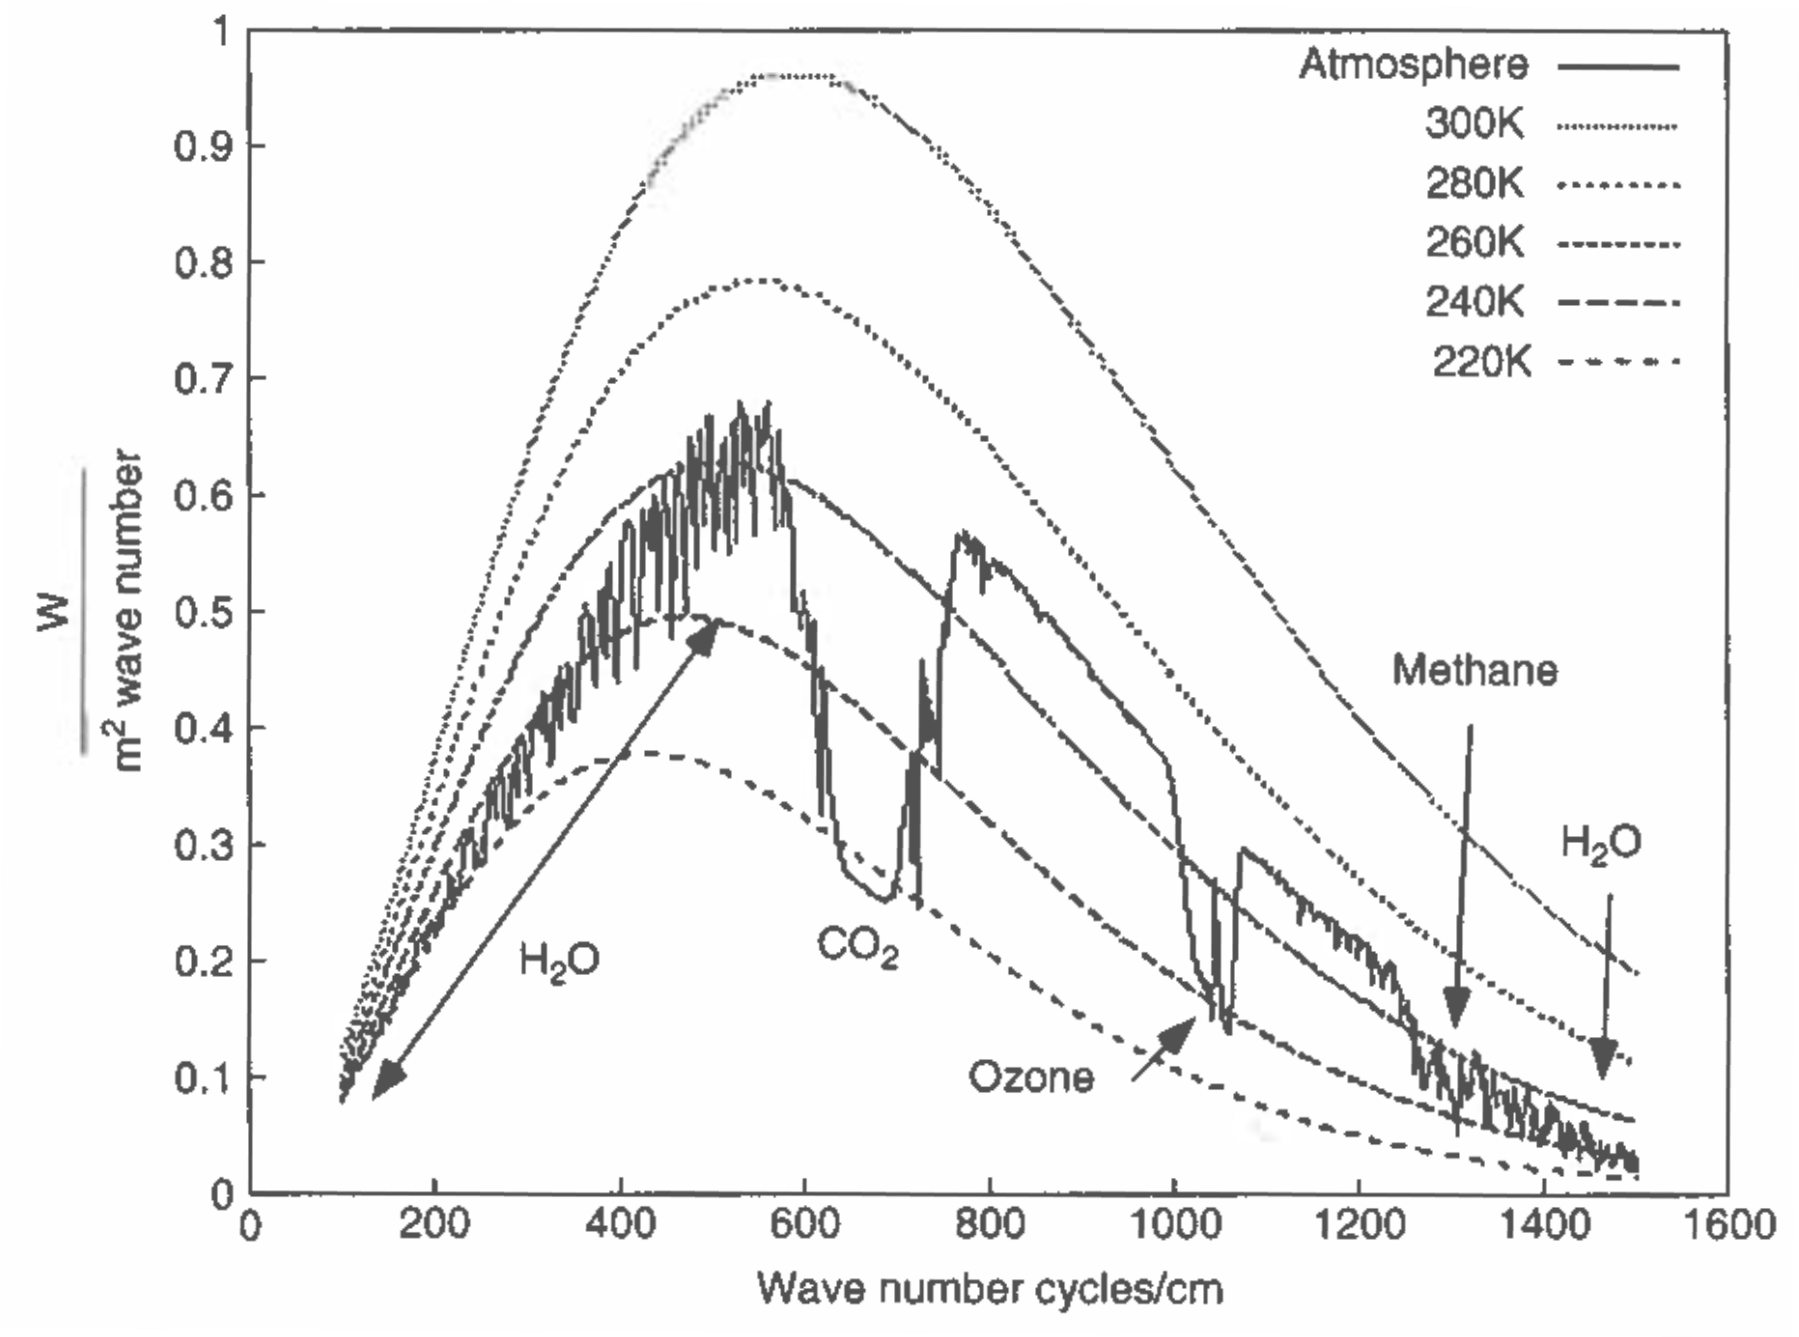
\includegraphics[width=0.95\textwidth]{images/archer_fig-4-3_rotated.png}
\end{center}

\end{frame}
%%%%%%%%%%%%%%%%%%%%%%%%%%%%%%%%%%%%%%
\begin{frame}{Blackbody curves, increasing $\text{CO}_2$}

\begin{center}
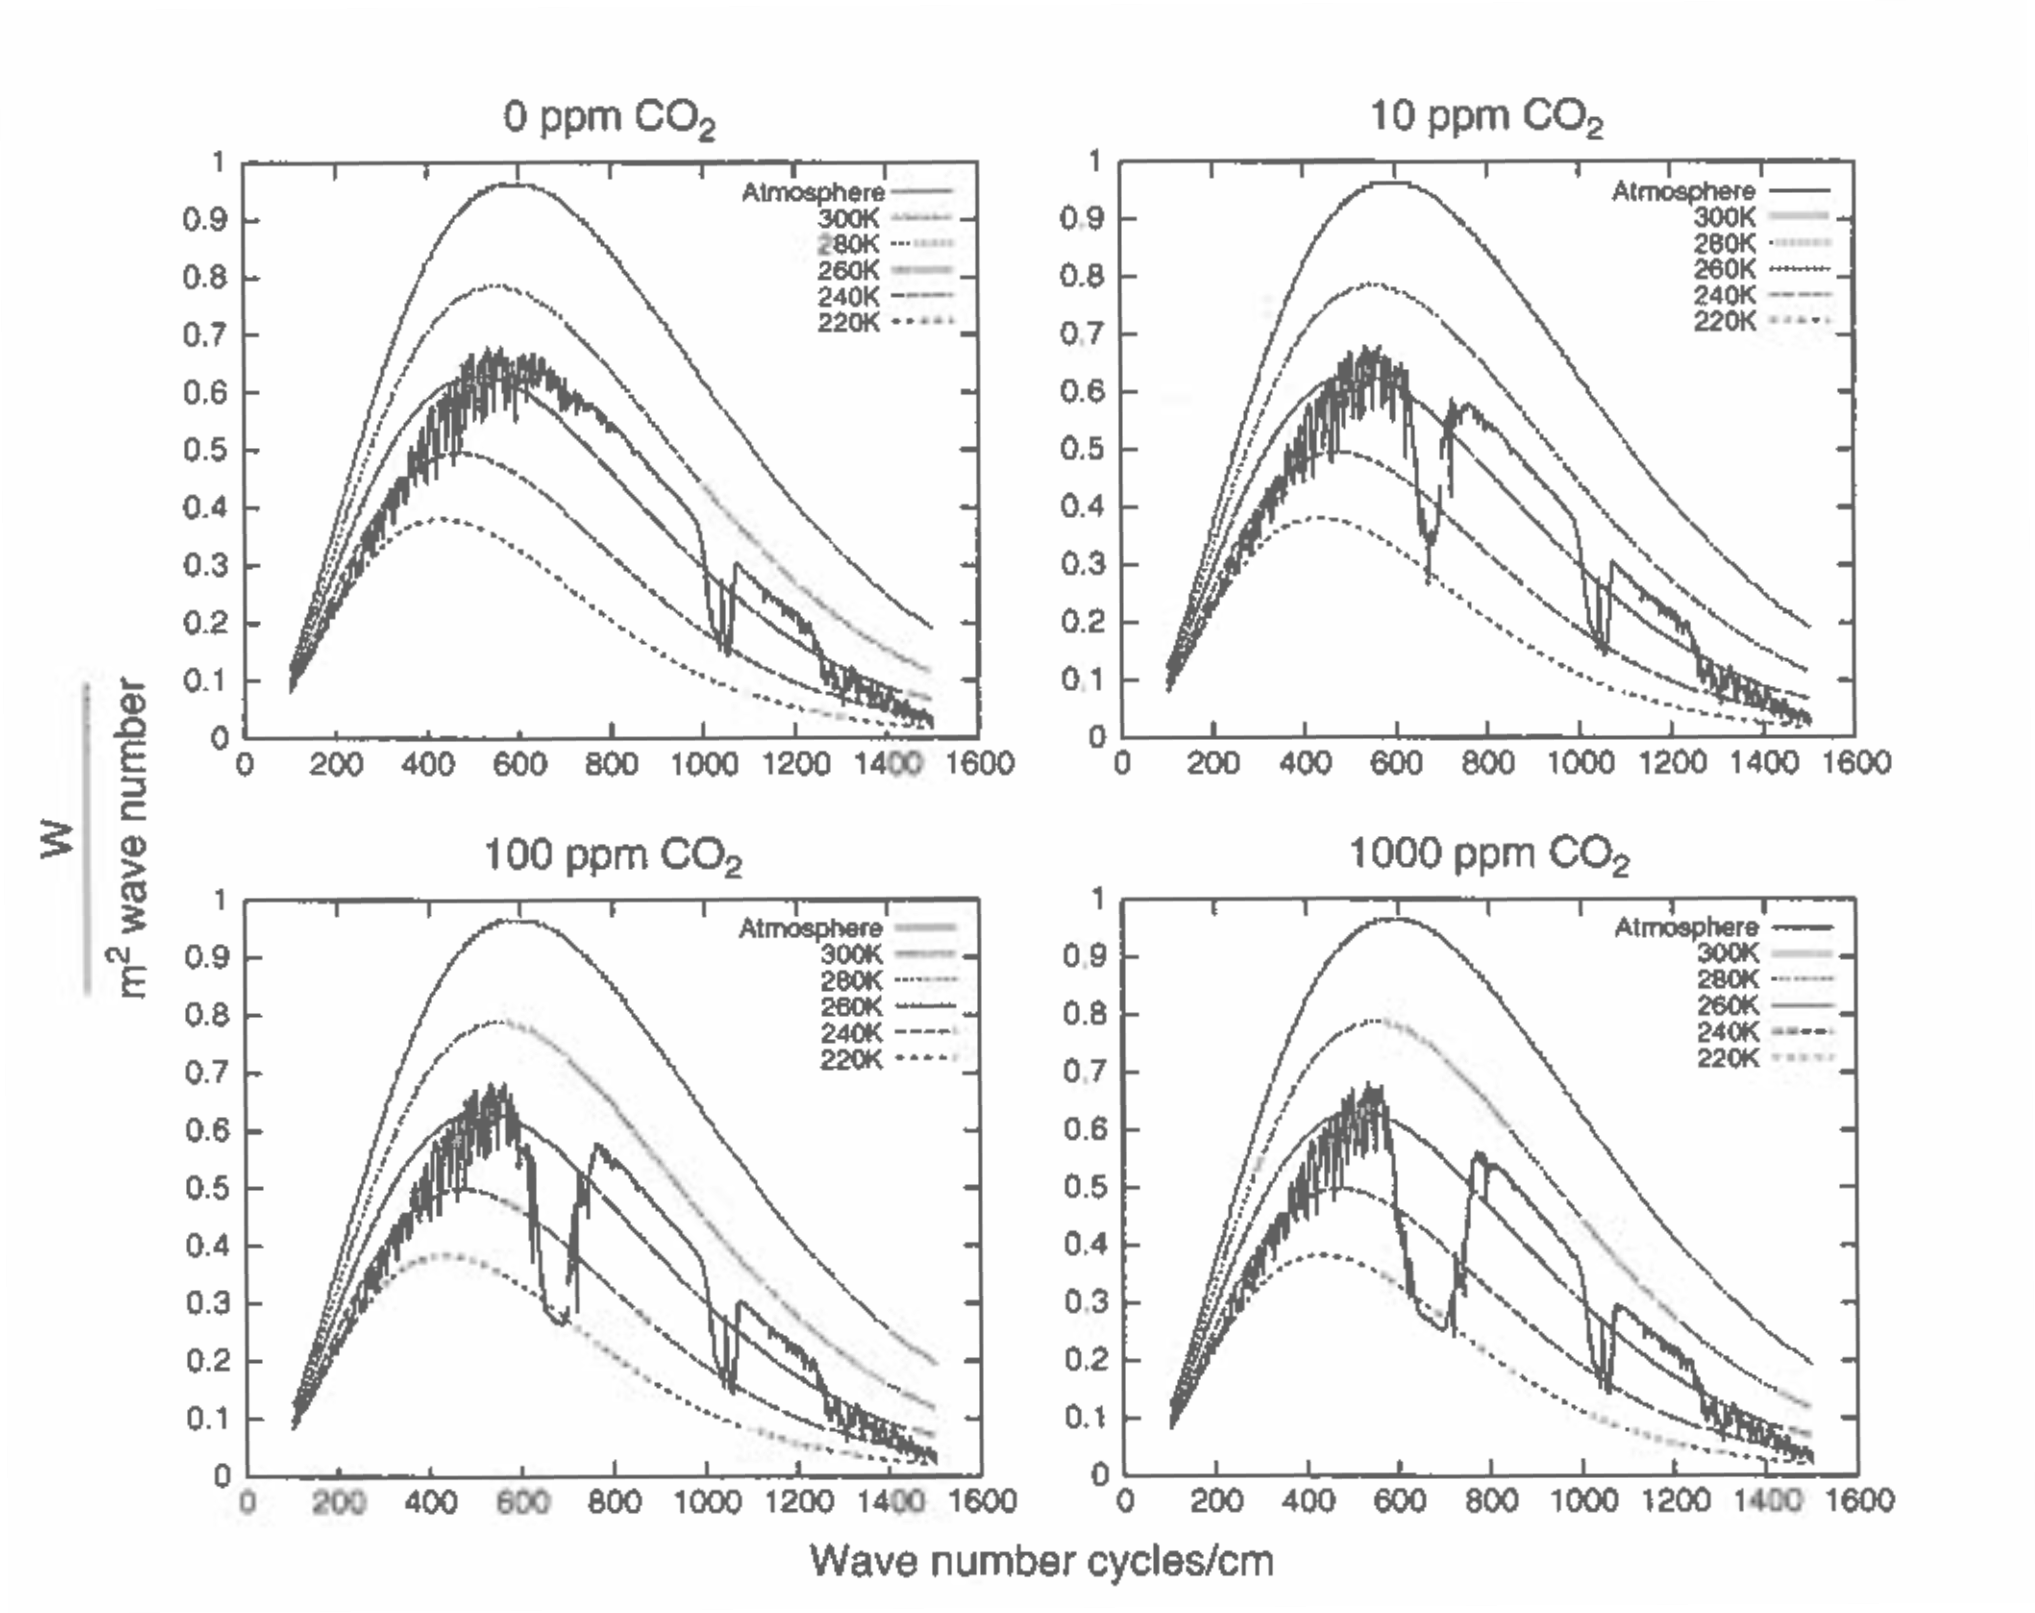
\includegraphics[width=0.95\textwidth]{images/archer_fig-4-5_rotated.png}
\end{center}

\end{frame}
%%%%%%%%%%%%%%%%%%%%%%%%%%%%%%%%%%%%%%
\begin{frame}{Increasing $\text{CO}_2$ and lost power}

\begin{center}
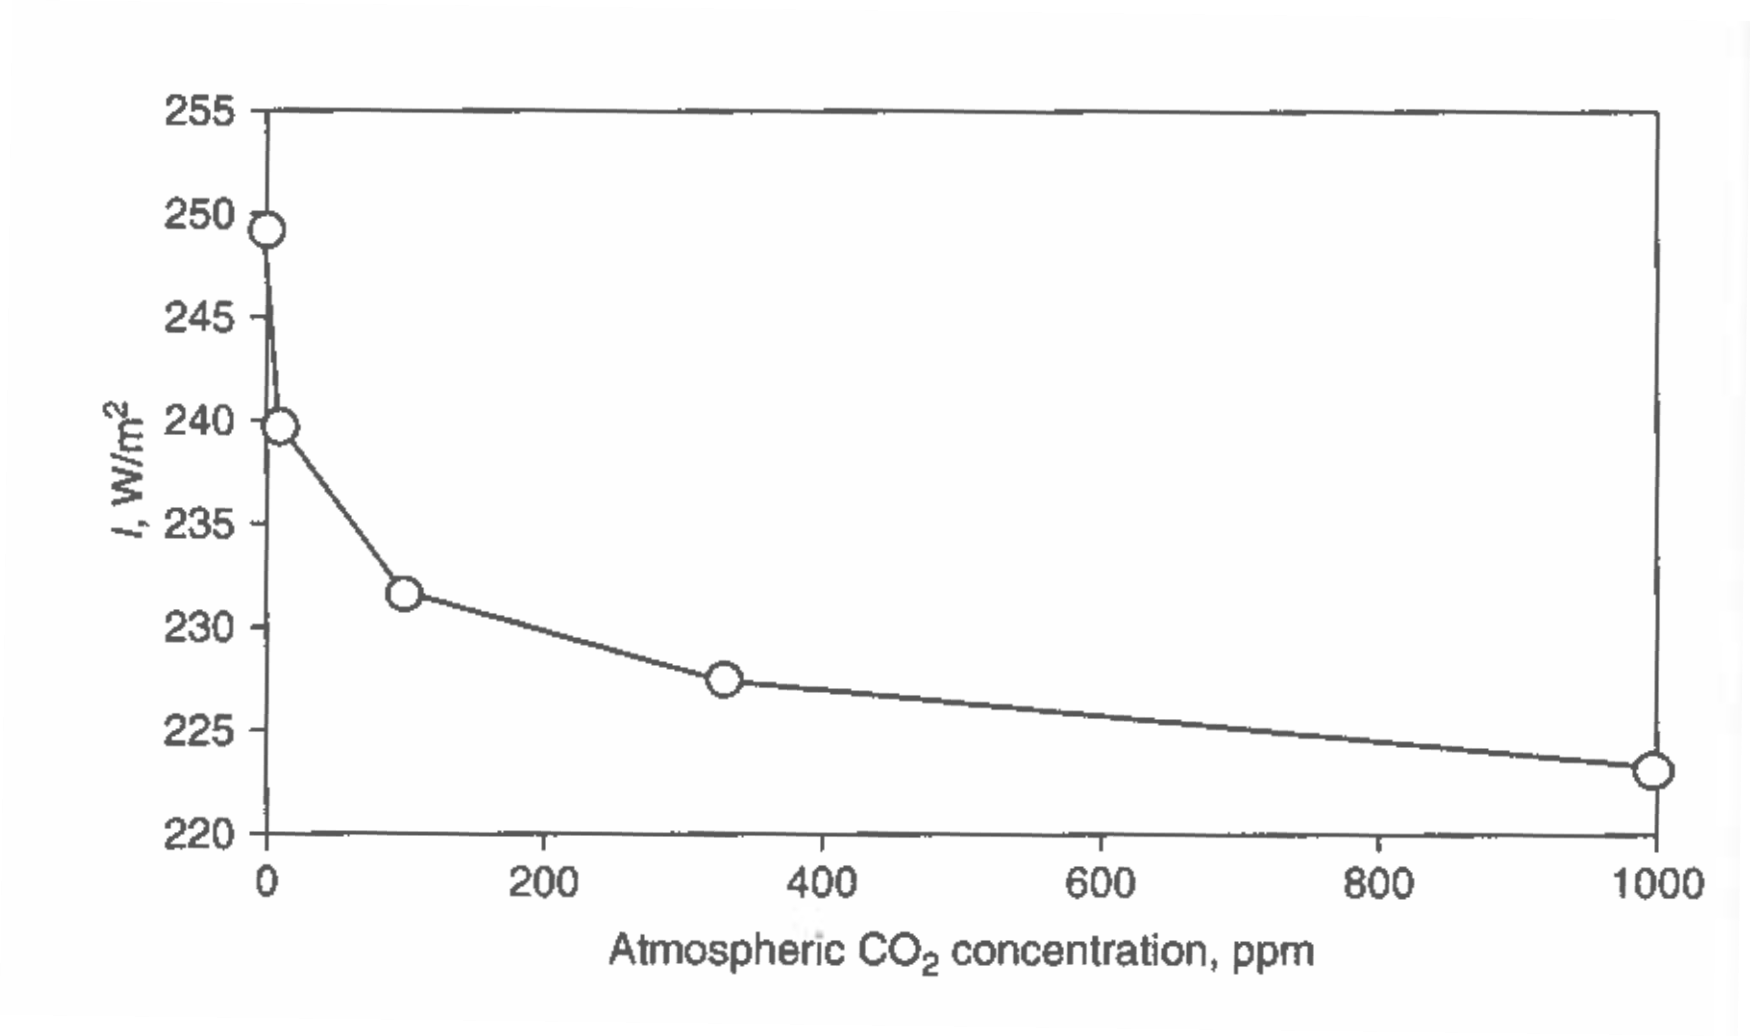
\includegraphics[width=\textwidth]{images/archer_fig-4-6_rotated.png}
\end{center}

\end{frame}
%%%%%%%%%%%%%%%%%%%%%%%%%%%%%%%%%%%%%%
\end{document}
